\documentclass{article}
\usepackage{tikz}
\usepackage{pgfplots}
\pgfplotsset{compat=1.18}
\usepackage{amsmath}
\usepackage{amssymb}
\usepackage{dsfont}
%\usepackage{txfonts}

% eisenstein integers are of the form a+b\omega where \omega = \frac{-1 + i\sqrt{3}}{2}
% -1/2 + \sqrt{3}/2 i

\newcommand{\set}[1]{\{#1\}}

\DeclareMathOperator{\rmd}{d}
\DeclareMathOperator{\abs}{abs}

\pgfmathparse{sqrt(3)/2}
\edef\sqthreeotwo{\pgfmathresult}

\def\eisToCar#1#2{
  \edef\a{#1}
  \edef\b{#2}
  \pgfmathparse{-\b/2}
  \edef\bwRe{\pgfmathresult}
  \pgfmathparse{\b*\sqthreeotwo}
  \edef\bwIm{\pgfmathresult}
  \pgfmathparse{\a+\bwRe}
  \xdef\currX{\pgfmathresult}
  \xdef\currY{\bwIm}%
}

%(0 -1) x   %% x -> -y
%(1  0) y   %% y -> x
\def\rotateNinety#1#2{ 
  \edef\x{#1}
  \edef\y{#2}
  \xdef\rotY{#1}
  \pgfmathparse{-#2}
  \xdef\rotX{\pgfmathresult}
  }

\gdef\one{1}
\gdef\zero{0}

\def\writeb#1{\pgfmathparse{#1 >= 0}\ifx\pgfmathresult\one+#1\else#1\fi}

% an eisenstein integer a+b\omega is manhattan distance d(a+b\omega) from 0
% d(a+b\omega) = abs(a) + abs(b) if ab <= 0
% d(a+b\omega) = max(abs(a), abs(b)) if ab > 0

\xdef\maxSteps{4}

\pgfmathparse{sqrt(3)}
\xdef\sqthree{\pgfmathresult}

\gdef\testInGrid#1#2#3{
  \pgfmathparse{#1*#2 <= 0}
  \edef\oppSign{\pgfmathresult}
  \ifx\oppSign\one
  \pgfmathparse{abs(#1) + abs(#2)}
  \else\pgfmathparse{max(abs(#1), abs(#2))}
  \fi
  \edef\manhattanDist{\pgfmathresult}
  \pgfmathparse{\manhattanDist <= #3}
  \xdef\withinGrid{\pgfmathresult}
}

\begin{document}
The Eisenstein integers are of the form $a + b\omega$, where $\omega = \frac{-1 + i\sqrt{3}}{2}$. They form a triangular lattice and the ring $\mathds{Z}[\omega]$.

A triangle can be represented as the set of three Eisenstein integers which surround its center. E.g., $\set{0, 1, 1+\omega}$ coresponds to the triangle highlighted orange below.
\[
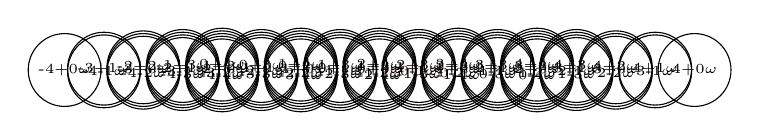
\begin{tikzpicture}
      \eisToCar{1}{1}
  \filldraw[orange!25] (0,0)--(1,0)--(\currX,\currY)--cycle;
    \foreach \a in {-5, ..., 5}{
    \foreach \b in {-5, ..., 5}{
      \testInGrid{\a}{\b}{\maxSteps}
      \ifx\withinGrid\one
      \eisToCar{\a}{\b}
      \rotateNinety{\currX}{\currY}
      %% \filldraw[color=blue!50] (\rotX/\sqthree,\rotY/\sqthree) circle (.1);      
      \else\fi
      }
    }
    
  \foreach \a in {-5, ..., 5}{
    \foreach \b in {-5, ..., 5}{
      \testInGrid{\a}{\b}{\maxSteps}
      \ifx\withinGrid\one
      \eisToCar{\a}{\b}
      \draw (\currX,\currY) circle (.4625);
      \draw node at (\currX,\currY) {\tiny $\scriptscriptstyle\text{\a\writeb\b}\omega$};      
      \else\fi
      }
  }
\end{tikzpicture}
\]
The manhattan distance of an Eisenstein integer from the origin is\footnote{It doesn't matter which one is the ``or equal to'' comparison. If one of $a$ or $b$ is zero $|a| + |b| = \max(|a|, |b|)$.}
\[
\rmd(a + b\omega) =
\begin{cases}
  |a| + |b| &\text{if } ab \le 0\\
  \max(|a|, |b|) &\text{if } ab > 0.
  \end{cases}
\]
When a and b are of opposite signs, $a$ and $b$ individually contribute to the number of steps moved. But when $a$ and $b$ are the same sign, each multiple of $1+1\omega$ corresponds to \textit{just one step}, not two. After removing all the multiples of $1+1\omega$, one of $a$ or $b$ will be zero, and the abolute value of the nonzero component contributes the remaining steps. Putting this thought process into algebra reveals that the manhattan distance when $a$ and $b$ are the same sign is
\begin{align*}
  \rmd(a + b\omega) ={}& \min(|a|, |b|) && \text{(multiples of $1+1\omega$)}\\
  & + \max(|a|, |b|) - \min(|a|, |b|) && \text{(remaining steps after factoring out all $1+1\omega$)}\\
  ={}& \max(|a|, |b|)
\end{align*}
\end{document}
